\documentclass[a4paper,abstracton]{scrreprt}
\usepackage[T1]{fontenc}
\usepackage[utf8]{inputenc}
\usepackage[ngerman]{babel}
\usepackage{pdfpages} 

%correct linebreaking in bibliography
\usepackage{hyperref}
\usepackage{breakurl}

%lists
\usepackage{mdwlist}

%biblatex
\usepackage[babel,german=quotes]{csquotes}
\usepackage[style=authortitle]{biblatex}
%\bibliography{bib}
\bibliography{test}

\usepackage{filecontents}

\begin{filecontents}{test.bib}
@Electronic{entoloma,
  Title                    = {Roetlinge / Entoloma},
  Author                   = {Machiel Evert Noordeloos},
  Url                      = {http://www.entoloma.nl/html/duits.html},
  Keywords                 = {entoloma},
  Owner                    = {Kevin},
  Urldate				   = {2014-07-03}
}
@Electronic{beschreibung,
  Title                    = {Rötling, Entoloma},
  Author                   = {R. Winkler},
  Url                      = {http://www.pilze.ch/pilzbestimmung/artenlisten/Entoloma.htm},
  Keywords                 = {beschreibung},
  Owner                    = {Kevin},
  Urldate				   = {2014-07-03}
}
\end{filecontents}

%table 
\usepackage{pbox}
\usepackage{booktabs}

%set numeration depth
\setcounter{secnumdepth}{3}
%set how many numbers show up in table-of-contents
\setcounter{tocdepth}{2}

\begin{document}
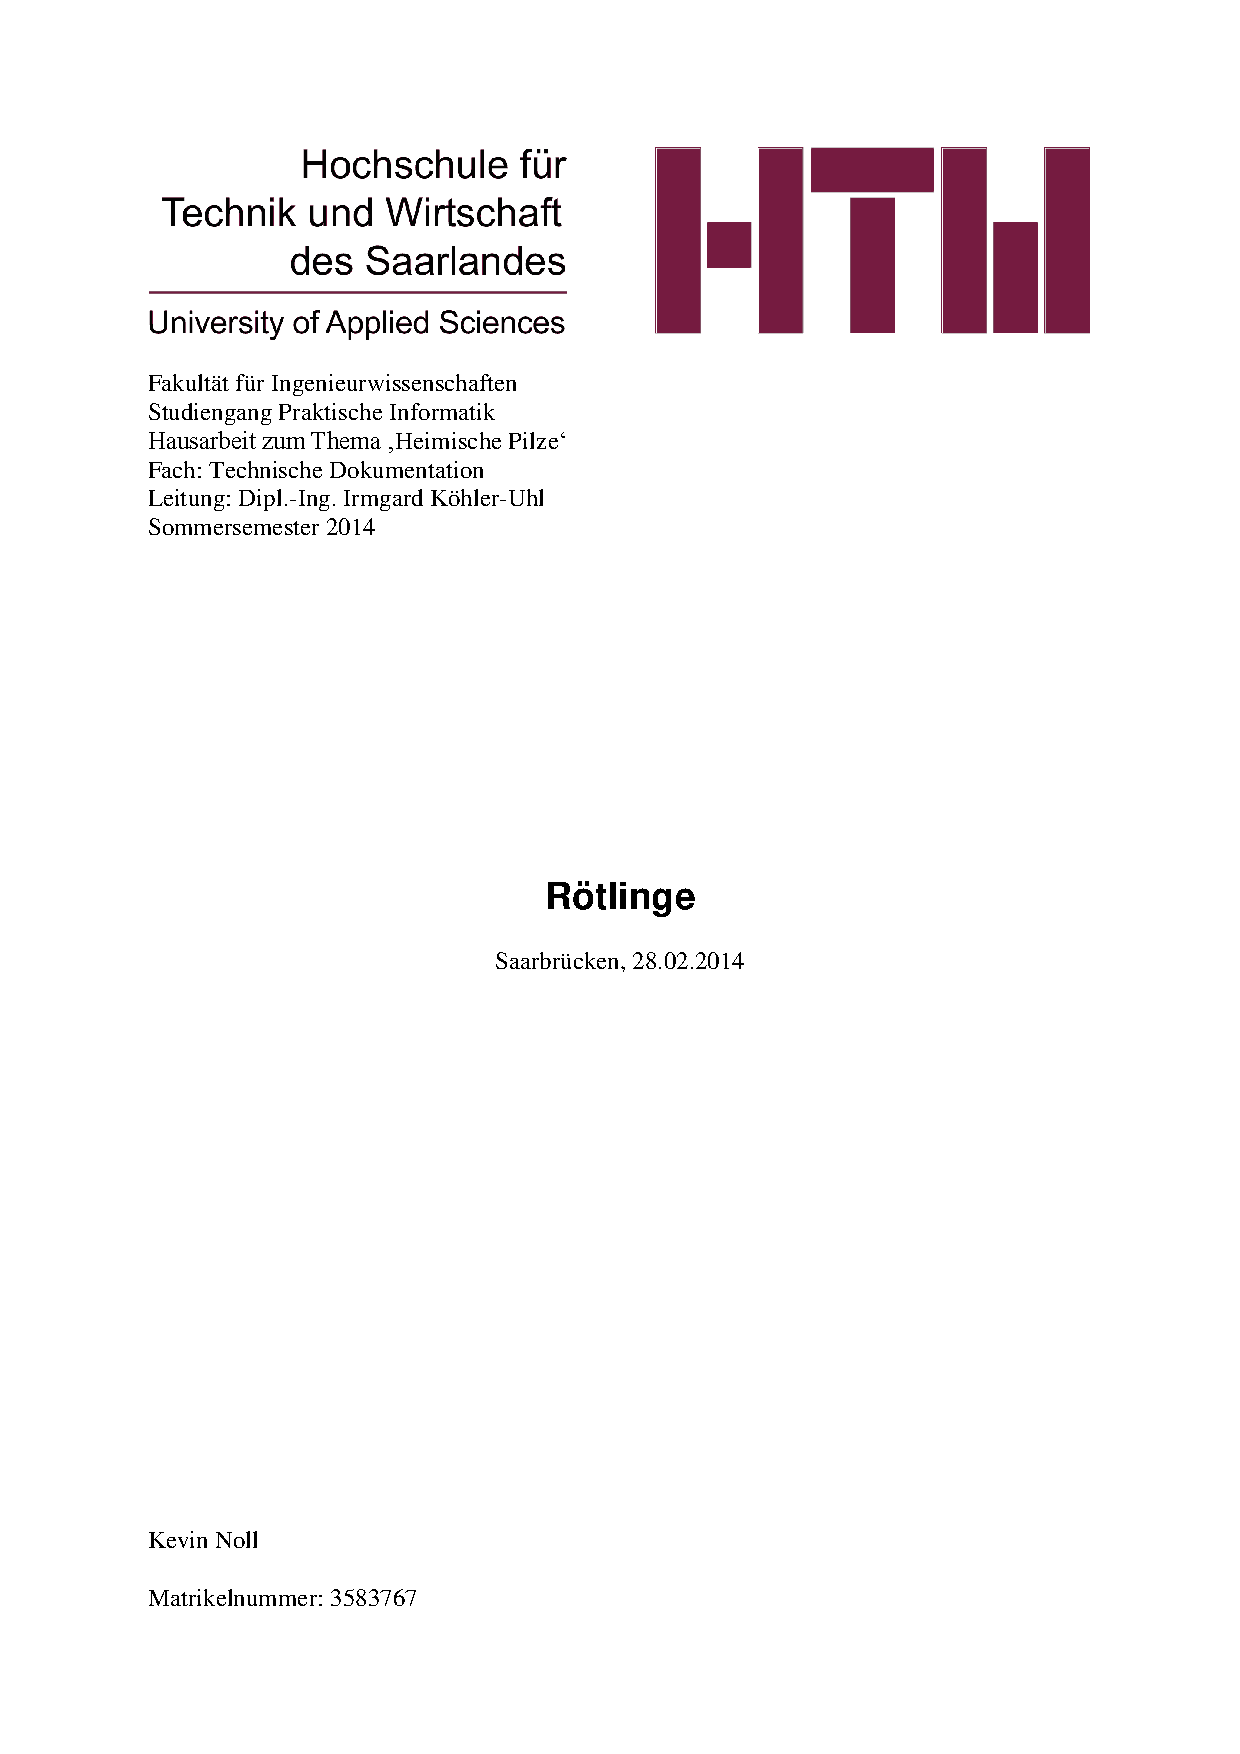
\includepdf[]{deckblatt.pdf}

%\author{Kevin Noll}
%\subject{Pilze und so}
%\title{Roetlinge, yo}
%\publishers{htwsaar}
%\maketitle
\tableofcontents
%\listoffigures
%\listoftables

\begin{abstract}
\begin{quote}%abstand rechts und links
Diese Arbeit befasst sich mit Pizlen und so nem kram. kein scheiss
\end{quote} 
\end{abstract}

\chapter{Vorwort}
Diese Ausarbeitung ist Bestandteil einer Reihe von Ausarbeitungen, die im Zuge der Vorlesung "'Technische Dokumentation"' entstanden sind. Der Kerngedanke bei der Anfertigung dieser Arbeit ist, zu erlernen, wie man mit fachbezogenen Texten umgeht -- von der Recherche über die Erstellung bis hin zur Anfertigung eines korrekten Literaturverzeichnisses. Unter dem Schirmthema \emph{Heimische Pilze} beschäftigt sich diese Ausarbeitung mit den Rötlingen (lat.: "'Entoloma"'). Es werden unter anderem Kenntnisse über die benötigte Bodenbeschaffenheit, die Beschreibung des Pilzes, die bei Pilzen so wichtigen Verwechslungsmöglichkeiten sowie die Zubereitung vermittelt.
\chapter{Rötlinge}
\section{Allgemeines}
Rötlinge (lat.: "'Entoloma"') sind eine direkte Untergruppe -- auch Gattung genannt -- der Familie der Rötlingsverwandten (lat.: "'Entolomataceae"'). Wie alle Arten der Rötlingsverwandten besitzen die Rötlinge rosa- bis braunfarbenes Sporenpulver. Die Sporen der Rötlinge sind dabei im Gegensatz zu vielen anderen Gattungen der Familie eckig, was jedoch nur unter einem Mikroskop ersichtlich ist. Weiterhin besitzen viele Arten der Rötlinge sogenannte Zystiden. 
\footcite{entoloma}
\section{Bodenbeschaffenheit}

\section{Beschreibung}
Rötlinge kommen mit kleinen bis großen Fruchtkörpern in vielen verschiedenen Farben und Formen vor. Die Formen des Hutes der Rötlinge reichen von glockig-kebelig über breitgebuckelt, gewölbt, mit oder ohne Papille bis zu genabelt oder trichterig. Die Farbe des Fruchtkörpers kann dabei unterschiedlichster Art sein, erscheint jedoch meist in grauen bis braunen Tönen von blass bis sehr dunkel. Manche Gattungsanhänger bilden jedoch auch intensive Blautöne aus, selten können auch Grüntöne oder Rosatöne gefunden werden. 

Die Oberfläche des Pilzhutes ist im Normalfall metallisch glänzend, in selteneren Fällen jedoch auch filzig, faserig oder etwas schuppig. die Lamellen sind durch das bereits erwähnte rosafarbene Sporenpulver dementsprechend gefärbt.
\footcite{beschreibung}

\section{Versuch der Aufteilung in mehrere Gattungen}
\section{Verwechslungsmoeglichkeiten}
\section{Inhaltsstoffe, Geniessbarkeit}
\section{Unterarten}
\subsection{PILZ A}
\subsection{PILZ B}
\subsection{PILZ C}
\subsection{PILZ D}
\section{Verwendung und Zubereitung mit Rezept}

%sadfsdf
\printbibliography


\end{document}